Behaviour of all entities within the game are discussed in this section.

\subsection{Structure}\label{subsec:behaviourStructure}
We have chosen to use goal-driven behaviour in our game.
Three main classes make up most of the structure, they are: \textit{Goal}, \textit{CompositeGoal} and \textit{AtomicGoal}.
As seen in the naming, a composite design pattern has been used to enable the grouping of goals while keeping the same functionalities.
This means that an \textit{AtomicGoal} can be used in the same way as a \textit{CompositeGoal} with the exception of \textit{AddSubGoal()},
which is only implemented in the composite.
This structure is used to create all strategy-level goals.

The class diagram below (fig.\ref{fig:behaviourClassDiagram}) shows the structure.

\begin{figure}[h!]
    \begin{center}
        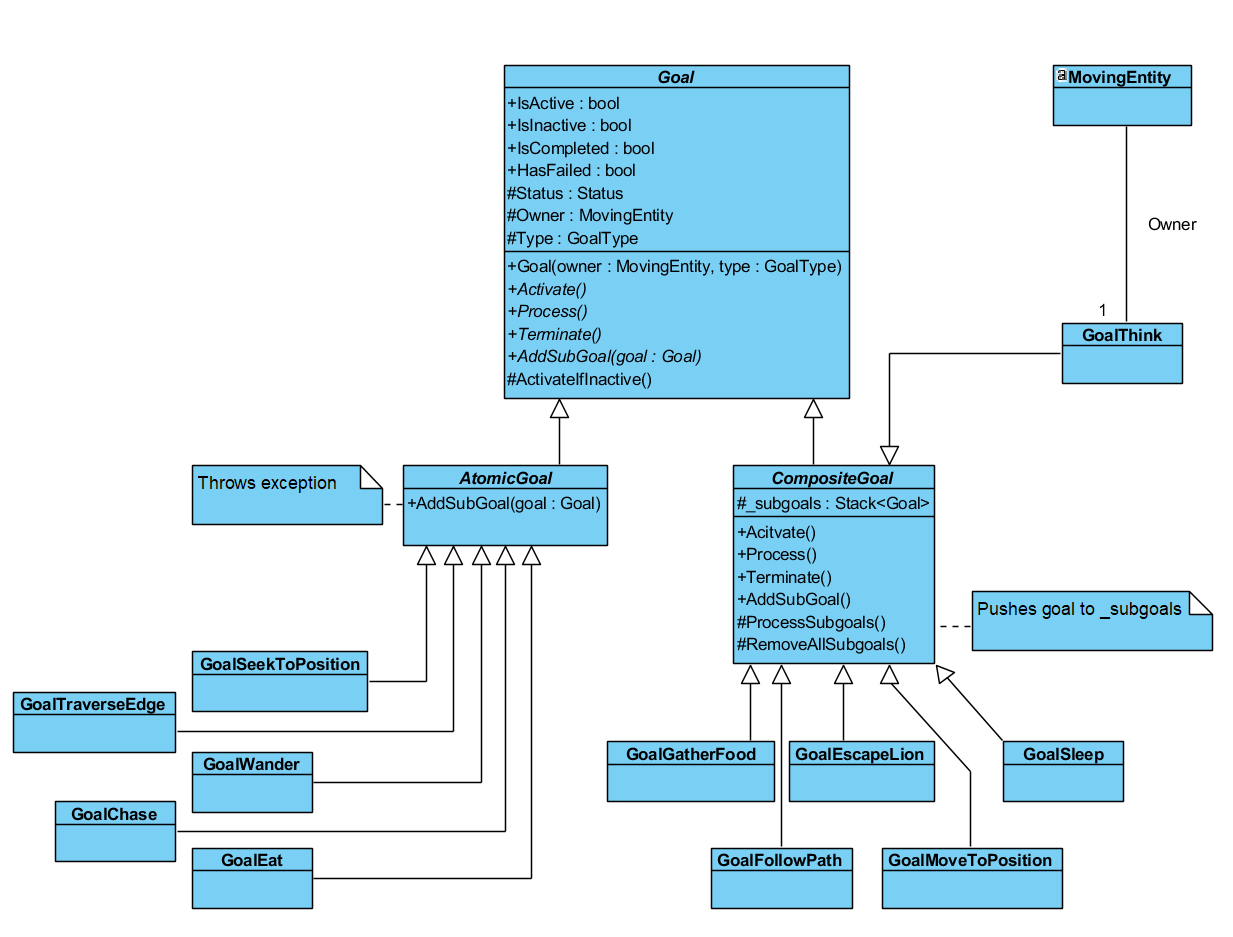
\includegraphics[width=28em]{Goals.jpg}
    \end{center}
    \caption{Goals class diagram}
    \label{fig:behaviourClassDiagram}
\end{figure}


\subsection{Goals}\label{subsec:behaviourGoals}
To give each entity a specific behaviour, we have created a couple of (composite) goals with some underlying atomic goals.
These goals wil be discussed below.

\subsubsection{Gather Food}\label{sec:behaviourFood}
Search for food
eat food
Lion and Gazelle
Lion -> Chase Gazelle

\subsubsection{Escape From Lion}\label{sec:behaviourEscape}
Gazelle

\subsubsection{Sleep}\label{sec:behaviourSleep}
Lion sleeps tonight -> Gazelle very happy

